\chapter{Materiais e Métodos} \label{sec:mat&met}

No presente capítulo introduz-se o conjunto de metodologias utilizadas ao longo do trabalho para a construção das análises e dos resultados obtidos em ambos os estudos de caso apresentados nos Capítulos \ref{sec:EstCasoAmbev} e \ref{sec:EstCasoAmazon}.
Partes das  metodologias utilizadas no trabalho já foram descritas no Capítulo \ref{sec:revis_biblio} como partes das referências conceituais utilizadas no trabalho. Assim, serão devidamente referenciados sempre que utilizados.
Por outro lado, parte das metodologias desenvolvidas foram construídas para o desenvolvimento do presente trabalho, tornando conveniente a explicação das motivações e hipóteses adotadas.

Na Seção \ref{sec:variaveis_do_problema} inicia-se o capítulo a partir da quantificação do problema estudado através de variáveis mensuráveis nos estudos de caso.
Tal seção tem como objetivo estabelecer a base das análises realizadas nos estudos de caso.

Posteriormente, na Seção \ref{sec:ferramentas}, apresenta-se as ferramentas utilizadas ao longo do trabalho, tais como a linguagem de programação \textit{Python}, os softwares de análise georreferenciada \textit{QGIS} e \textit{GeoDa} e, por fim, o editor de planilhas digitais \textit{Excel}.

Adiante, na Seção \ref{sec:dados_de_informacao_geografica}, são apresentadas as bases de dados georreferenciadas utilizadas para a concepção de algumas análises. Entre elas, cita-se os mapas georreferenciados dos bairros de cada cidade estudada nos estudos de caso. A seguir, na Seção \ref{GeoDa}, apresenta-se as metodologias utilizadas dentro da ferramenta \textit{GeoDa} para a construção das análises geoestatísticas realizadas. Em seguida, na Seção \ref{sec:dispGeoRotas} apresenta-se a metodologia desenvolvida para a análise da dispersão geográfica das rotas, que, em suma, busca avaliar o posicionamento dos PDE em relação aos outros PDEs da mesma rota de entregas.

Por fim, na Seção \ref{BibLMRA}, apresenta-se a concepção de toda a metodologia utilizada em \textit{Python} para a construção da biblioteca \textit{Last-Mile-Routing-Analyzer}. Essa biblioteca, publicada abertamente na plataforma Github (\citeauthoronline{guilherme_fernandes_alves_2022_6792977}, \citeyear{guilherme_fernandes_alves_2022_6792977}), é responsável por um conjunto de procedimentos, desde a abertura e organização das bases de dados, até análises relativas à estrutura viária.

Ademais, é possível definir as hipóteses preliminares que foram estabelecidas no início do projeto.
Estas premissas foram importantes para que o trabalho tivesse ao menos um direcionamento quanto às linhas de pesquisa que deveriam ser aprofundadas durante execução do trabalho.
%
\begin{enumerate}
    \item A configuração das vias pode fazer das cidades lugares mais ou menos complexos para entregas de distribuição de última milha, sendo que as condições de terreno também podem afetar essa complexidade (relevo, elevação, etc.);
    \item Por meio de abordagens vistas na literatura, será possível quantificar essas condições adversas de diferentes malhas urbanas, permitindo comparações baseadas em estatísticas e ao mesmo tempo facilitando investigações de correlações ou de relação causa x consequência;
    \item Verificar se regiões em que as rotas realizadas apresentam menor aderência ao sequenciamento programado apresentam também piores valores de fator de circuito ou outras medidas;
    \item Avaliar se, ao quantificar a malha viária de um centro urbano através de diferentes medidas, é possível inferir quais seriam as regiões de pior aderência ao sequenciamento programado. 
\end{enumerate}

Espera-se que ao final do trabalho possa se confirmar parcial ou completamente as hipóteses preliminares que foram descritos nesta seção.

%%%%%%%%%%%%%%%%%%%%%%%%%%%%%%%%%%%%%%%%%%%%%%
\section{Medidas da não aderência às roteirizações programadas} \label{sec:variaveis_do_problema}

Para se obter uma perspectiva quantitativa baseada em dados, foram definidas variáveis contínuas que representem a não aderência ao sequenciamento programado de entregas.
A partir dessas variáveis foi possível mensurar e analisar correlações entre medidas associadas à não aderência e qualquer outra medida escolhida, seja de ``circuicidade'', conectividade, ou outras.

Ademais, foi importante contar que as variáveis propostas puderam ser calculadas a partir das bases de dados históricos utilizadas no trabalho. 
Ademais, essas medidas foram simples o suficiente a ponto de permitir a quantificação do fenômeno de não aderência tanto para o caso da empresa de bebidas quanto para o caso da \textit{Amazon.com}.
Não obstante, espera-se que as medidas propostas poderão ser utilizadas também em trabalhos futuros que considerem estudos de casos similares, independente da empresa analisada.

A seguir, são descritas as três variáveis propostas para quantificar o fenômeno de não aderência: Repasse, Devolução e Não Aderência Sequencial (NAS).
Essas medidas foram utilizadas ao longo do trabalho para investigar se há alguma consistência ou recorrência de repasses em PDEs ou rotas específicas, a fim de se identificar regiões que deveriam receber maior atenção durante o planejamento de rotas de entregas.

%%%%%%%%%%%%%%%%%%%%
\subsection{Repasse}
 
Repasses são eventos inesperados que levam a equipe de entregas a realizar mais de uma visita ao mesmo PDE numa mesma rota. 
Em tais situações, identifica-se que por algum motivo a equipe é incapaz de realizar a entrega na primeira visita que realiza ao estabelecimento naquele dia.
Os repasses podem ocorrer por diversos motivos, dentre eles, destaca-se: o cliente estar ausente, o estabelecimento estar fechado (no caso de entregas B2B) e o cliente não possuir dinheiro suficiente para realizar o pagamento quando este é realizado durante a entrega (também B2B).

Deste modo, define-se a variável repasse como sendo o percentual de visitas, de acordo com a Equação \ref{eq:repasse}.
Nota-se que a medida de repasse pode ser calculada sobre um PDE, rota, área ou intervalo de tempo, assim permitindo diferentes análises a partir de uma única variável.
%
\begin{equation} \label{eq:repasse}
    Repasse (\%) = 100 \cdot \frac{n^{\circ} \; de \; repasses}{Total \; de \; entregas}
\end{equation}


%%%%%%%%%%%%%%%%%%%%%%
\subsection{Devolução}

Diferentemente do repasse, as devoluções acontecem quando a equipe de entregas, por alguma razão, não consegue realizar a entrega programada e acaba devolvendo as mercadorias para o CD.
Uma das causas de devoluções é a rejeição de mercadorias por parte do cliente, o qual pode identificar que o pacote não está em condições adequadas, ou que a entrega não contém exatamente os produtos que foram pedidos, ou até mesmo pode ser alegado que o endereço programado para entrega não corresponde ao endereço do cliente.
%
Outra causa das devoluções é a impossibilidade de entregas devido ao fim do expediente da equipe de entregas, muitas das vezes ocasionada por atrasos ocorridos em outras entregas da rota.

É possível definir uma variável de devolução como sendo o percentual de mercadorias (ou pacotes) devolvidas em relação ao total de mercadorias que deveriam ser entregues, conforme a Equação \ref{eq:devolucao}.
%
\begin{equation} \label{eq:devolucao}
    Devoluc\Tilde{a}o (\%) = 100 \cdot \frac{n^{\circ} \; de \; pacotes \; devolvidos}{Total \; de \; pacotes}
\end{equation}

%%%%%%%%%%%%%%%%%%%%%%%%%%%%%%%%%%%%%%%%%%%
\subsection{Não Aderência Sequencial (NAS)}

A terceira variável proposta é a Não Aderência Sequencial (NAS), que identifica os casos em que o pedido do PDE é entregue numa posição sequencial da rota diferente da planejada. 
Em exemplo, uma situação de NAS pode ser um caso em que a equipe de planejamento estabeleceu que determinado PDE seria a 4ª entrega de determinada rota mas, no instante da entrega, a operação opta por tornar o PDE o 6º a ser visitado naquele dia.

Nesse sentido, para cada entrega estabelece-se uma variável binária indicando se a entrega foi realizada na sequência programada ou não.
A partir daí, pode ser definida uma variável global de NAS como na Equação \ref{eq:NAS}.
%
\begin{equation} \label{eq:NAS}
    NAS(\%) = 100 \cdot \frac{n^{\circ} \; de \; etregas \; em \; sequencia \; diferente \; da \; programada}{Total \; de \; entregas} 
\end{equation}

%%%%%%%%%%%%%%%%%%%%%%%%%%%%%%%%%%%%%%%%%%%%%%
\section{Ferramentas} \label{sec:ferramentas} 

Ao longo do trabalho foram utilizados diversos recursos tecnológicos a fim de possibilitar o desenvolvimento das análises.
%
As ferramentas utilizadas configuram parte importante do conhecimento adquirido durante a graduação no curso de Engenharia Civil da Escola Politécnica.

Primeiramente destaca-se utilização da linguagem de programação \textit{Python} (\citeauthoronline{van1995python}, \citeyear{van1995python}) em sua versão 3.9, que permitiu a leitura de bases de dados e posterior tratamento das informações, representando parte importante da ciência de dados empregada durante o trabalho.
%
Além disso, ao utilizar rotinas escritas em linguagem \textit{Python} foi possível integrar dados provindos de banco de dados distintos por meio de bibliotecas dedicadas.
%
Destaca-se aqui a utilização das bibliotecas \textit{googlemaps} (versão 4.6.0) e \textit{osmnx} (versão 1.2.1), que permitem acesso às informações disponíveis nas plataformas \textit{Google Maps API}, e \textit{OpenStreetMap} (\citeauthoronline{OpenStreetMap}, \citeyear{OpenStreetMap}), respectivamente.
Com superior destaque para a \textit{OSMnx}, que também permitiu uma série de análises quanto à geometria e arranjo de diferentes malhas viárias.
% TODO: Falta uma citação do Google Maps aqui

No âmbito de sistemas de informações geográficas, foi utilizado o \textit{software} de código aberto \textit{QGIS} (\citeauthoronline{QGIS_software}, \citeyear{QGIS_software}), que é um aplicativo de código aberto que permite o tratamento de informações dados espaciais, bem como elaboração de mapas e representações dos dados georreferenciados.
Também foi utilizado o programa de código aberto \textit{GeoDa} (\citeauthoronline{anselin2010geoda}, \citeyear{anselin2010geoda}), que permitiu a aplicação de conceitos de geoestatística sobre os dados espaciais analisados.
 
Por fim, ressalta-se a importância do editor de planilhas digitais \textit{Excel} (\citeauthoronline{msexcel}, \citeyear{msexcel}), da empresa \textit{Microsoft}, que na presente pesquisa foi utilizado, essencialmente, para os procedimentos de armazenamento, tratamento, construção, análise e visualização de dados. 
Podendo estes dados ser referentes às bases fornecidas para os estudos de caso ou aos dados gerados a partir das análises. 

%%%%%%%%%%%%%%%%%%%%%%%%%%%%%%%%%%%%%%%%%%%%%%
\section{Dados de informação geográfica} \label{sec:dados_de_informacao_geografica}

%%%%%%%%%%%%%%%%%%%%%%%%%%%%%%%%%%%%%%%%%%%%%%%%%%%%%%%%%%%%%
\subsection{Guarulhos-SP, Brasil} \label{sec:georef_guarulhos}

Para elaboração do trabalho foi utilizado um arquivo em formato \textit{shapefile} contendo os limites de bairros da cidade de Guarulhos, que representa a maior parcela da região analisada no primeiro estudo de caso analisado.
%
Apesar de o CD da empresa atender também outras cidades como Itaquaquecetuba e Arujá durante a série histórica analisada, somente a cidade de Guarulhos foi selecionada para análises de mapeamento, uma vez que estas outras cidades carecem de dados mais acurados quanto aos limites de bairros e outras informações.

Este arquivo \textit{shapefile} tem sua origem no banco de dados da plataforma \textit{OpenStreetMap}, porém foi extraído através do \textit{software} \textit{QGIS} descrito na seção \ref{sec:ferramentas}. 
%
Após a sua obtenção, identificou-se um conjunto de falhas em sua composição.
%
Primeiro, identificou-se a presença de dois bairros localizados fora dos limites municipais de Guarulhos.
%
Em sequência, identificou-se que nove bairros estavam ausentes, formando espaços vazios no interior polígono e, por fim, dois dos bairros estavam com formatos inadequados quando comparados com um mapa da região.
%
Assim, através do \textit{QGIS} foi possível corrigir todos os problemas e, estabelecer uma base completa dos 47 bairros do município. 
%
A Figura \ref{fig:GRU_shapefile_QGIS} apresenta os bairros já corrigidos, enquanto que a Figura \ref{fig:GRU_shapefile} mostra como os dados estavam disponibilizados previamente.
%
Cita-se que para a construção dos bairros faltantes, utilizou-se como base as definições presentes no site da prefeitura local.
% TODO: citar essa fonte

\begin{figure}[htbp]
    \caption{Limites de bairros da cidade de Guarulhos}
    \begin{subfigure}{0.49\textwidth}
        \subcaption{Antes das correções}
        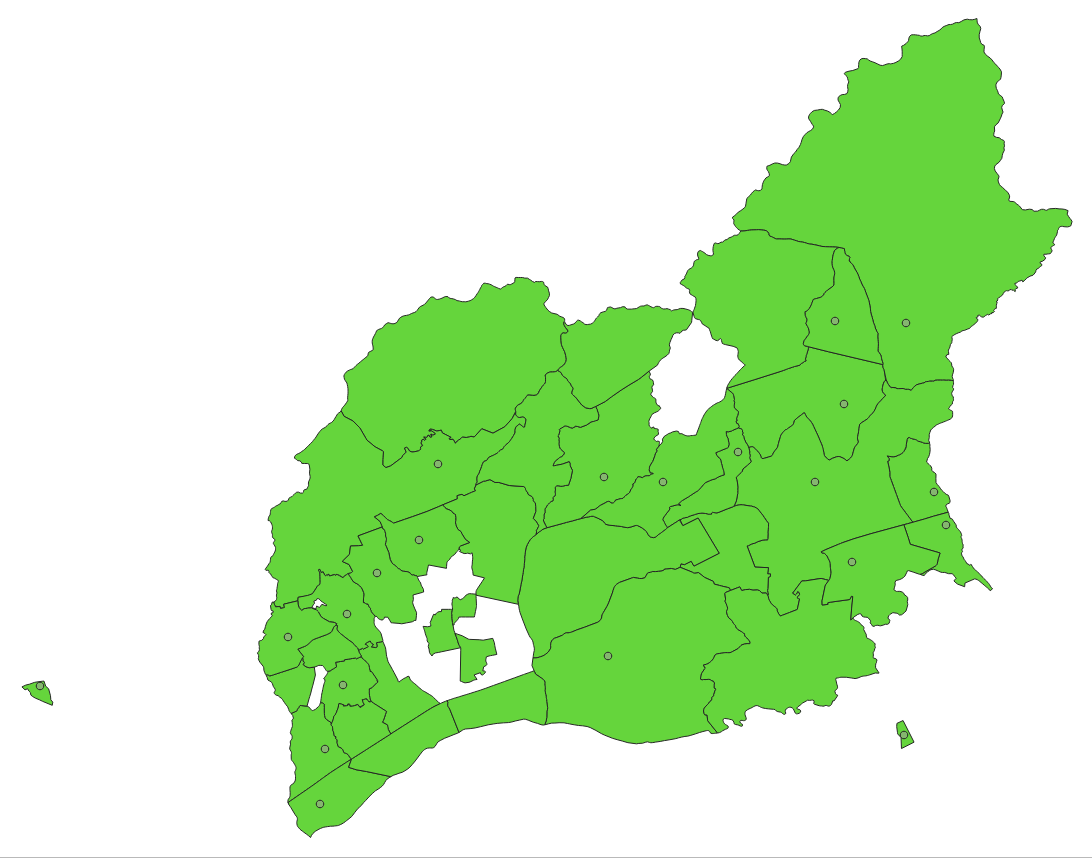
\includegraphics[height=0.75\textwidth]{images/4_materiais/gis/Guarulhos_SHAPE_QGIS.png}
        \label{fig:GRU_shapefile}
    \end{subfigure}
    \begin{subfigure}{0.49\textwidth}
        \subcaption{Após as correções}
        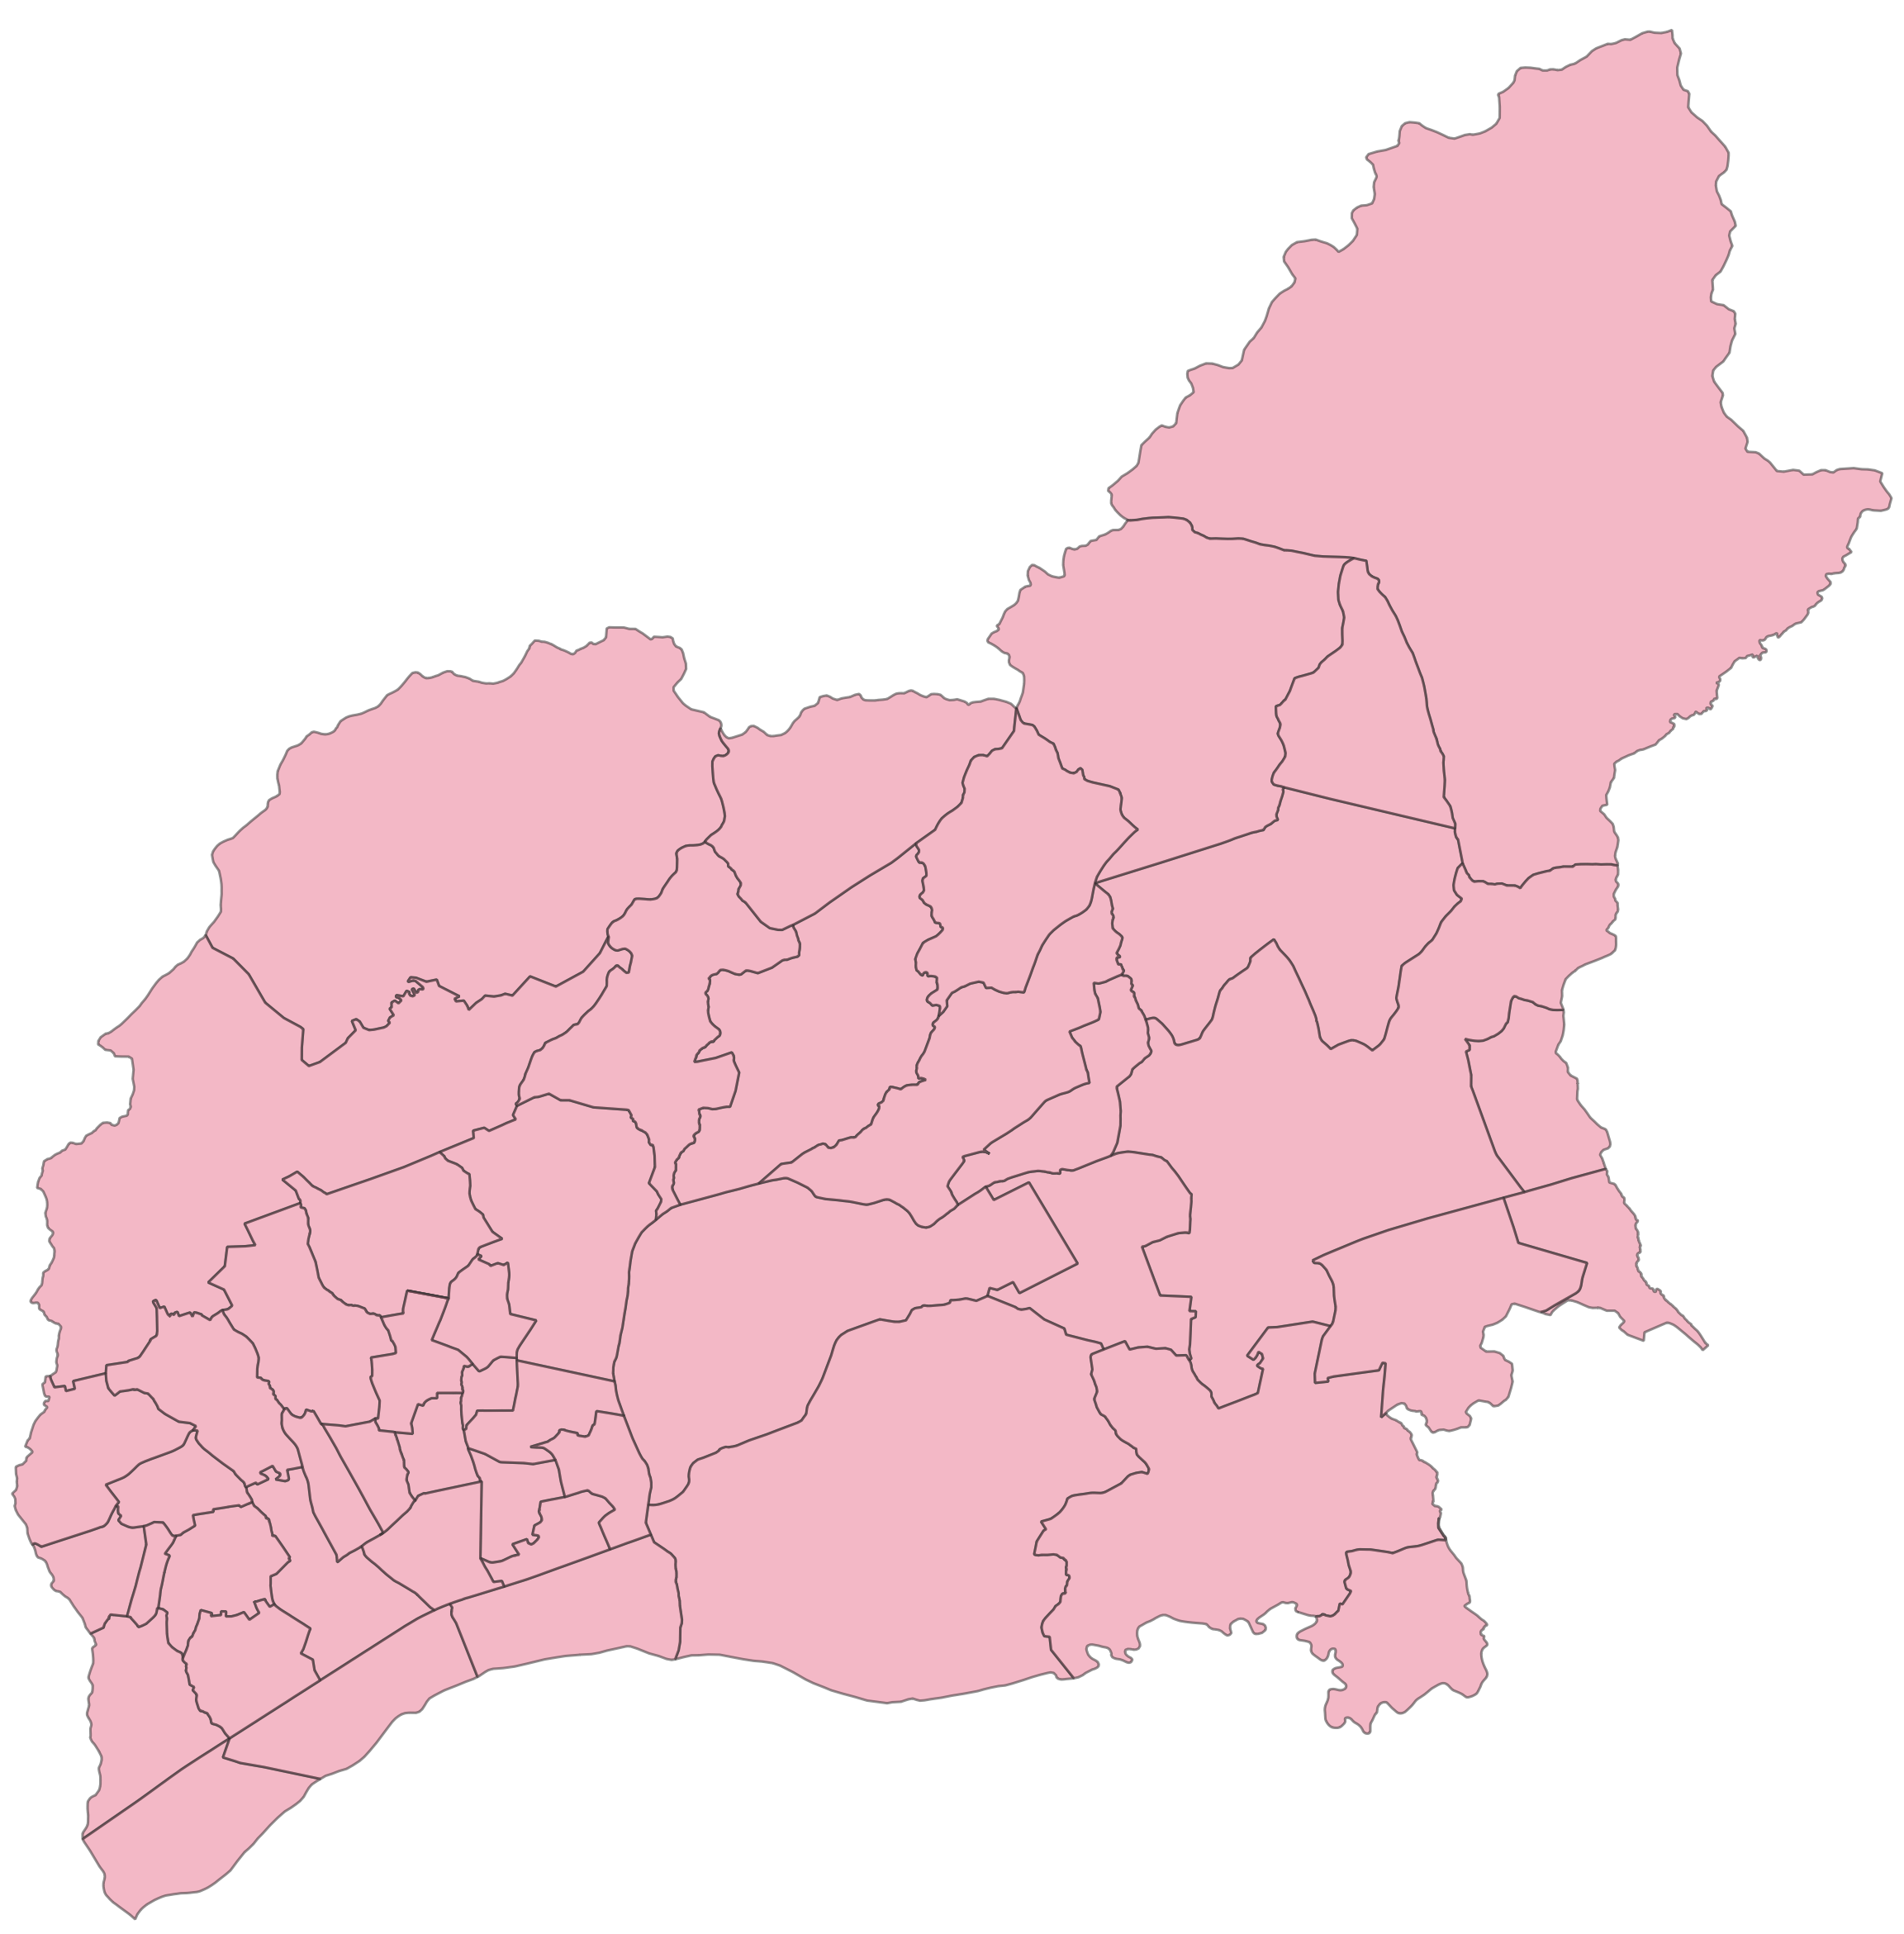
\includegraphics[height=0.75\textwidth]{images/4_materiais/gis/BairrosGuarulhosNovo.png}
        \label{fig:GRU_shapefile_QGIS}
    \end{subfigure}
    \centering
    \caption*{Fonte: Produzido pelos autores Fernandes \& Alves}
\end{figure}

A tabela \ref{tab:Bairros_shapefile}, disponível na seção \ref{sec:AppGIS}, traz o resumo do que se tem de informação deste arquivo \textit{shapefile} inicial que, no caso, são apenas o nome de cada bairro e sua área.

%%%%%%%%%%%%%%%%%%%%%%%%%%%%%%%%%%%%%%%%%%%%%%%%%%%%%%%%%%%
\subsection{Los Angeles, CA, Estados Unidos} \label{SIG_LA}

Na segunda parte do trabalho, em contraste a Guarulhos, é necessário que se obtenha dados georreferenciados das cinco cidades que compõe a operação amostrada da \textit{Amazon} na base de dados disponibilizada. 
%
Um grande enfoque do trabalho especialmente nas primeiras análises, porém, foi dado ao condado de Los Angeles, situado no Estado da Califórnia (EUA), devido à sua boa representatividade percentual da operação comparada às outras cidades.

Seguindo-se o mesmo procedimento do município de Guarulhos observado no tópico \ref{sec:georef_guarulhos}, buscou-se segregar a cidade em bairros para agrupar os dados da operação. 
%
Para tal, encontrou-se, nos arquivos públicos da Universidade do Sul da Califórnia (USC), um arquivo \textit{shapefile} atualizado dos polígonos que compõem cada bairro do município, como observado em \citeonline{USC2022}.
%
Diferentemente do caso de Guarulhos, o arquivo \textit{shapefile} de Los Angeles é composto por múltiplos bairros que não necessariamente apresentam atividade operacional da \textit{Amazon} e que, em geral, compreendem extensas áreas. 
%
Assim, visando o desempenho computacional de etapas futuras, selecionou-se apenas os polígonos dos bairros que continham, de fato, atividades operacionais da base de dados utilizada. 
%
Assim, resultou-se no polígono apresentado na Figura \ref{fig:bairros_LA}, que representa os bairros do condado de Los Angeles em cor branca (não selecionados) e azul (selecionados).

\begin{figure}[htbp]
    \centering
    \caption{Bairros de Los Angeles selecionados para análise}
    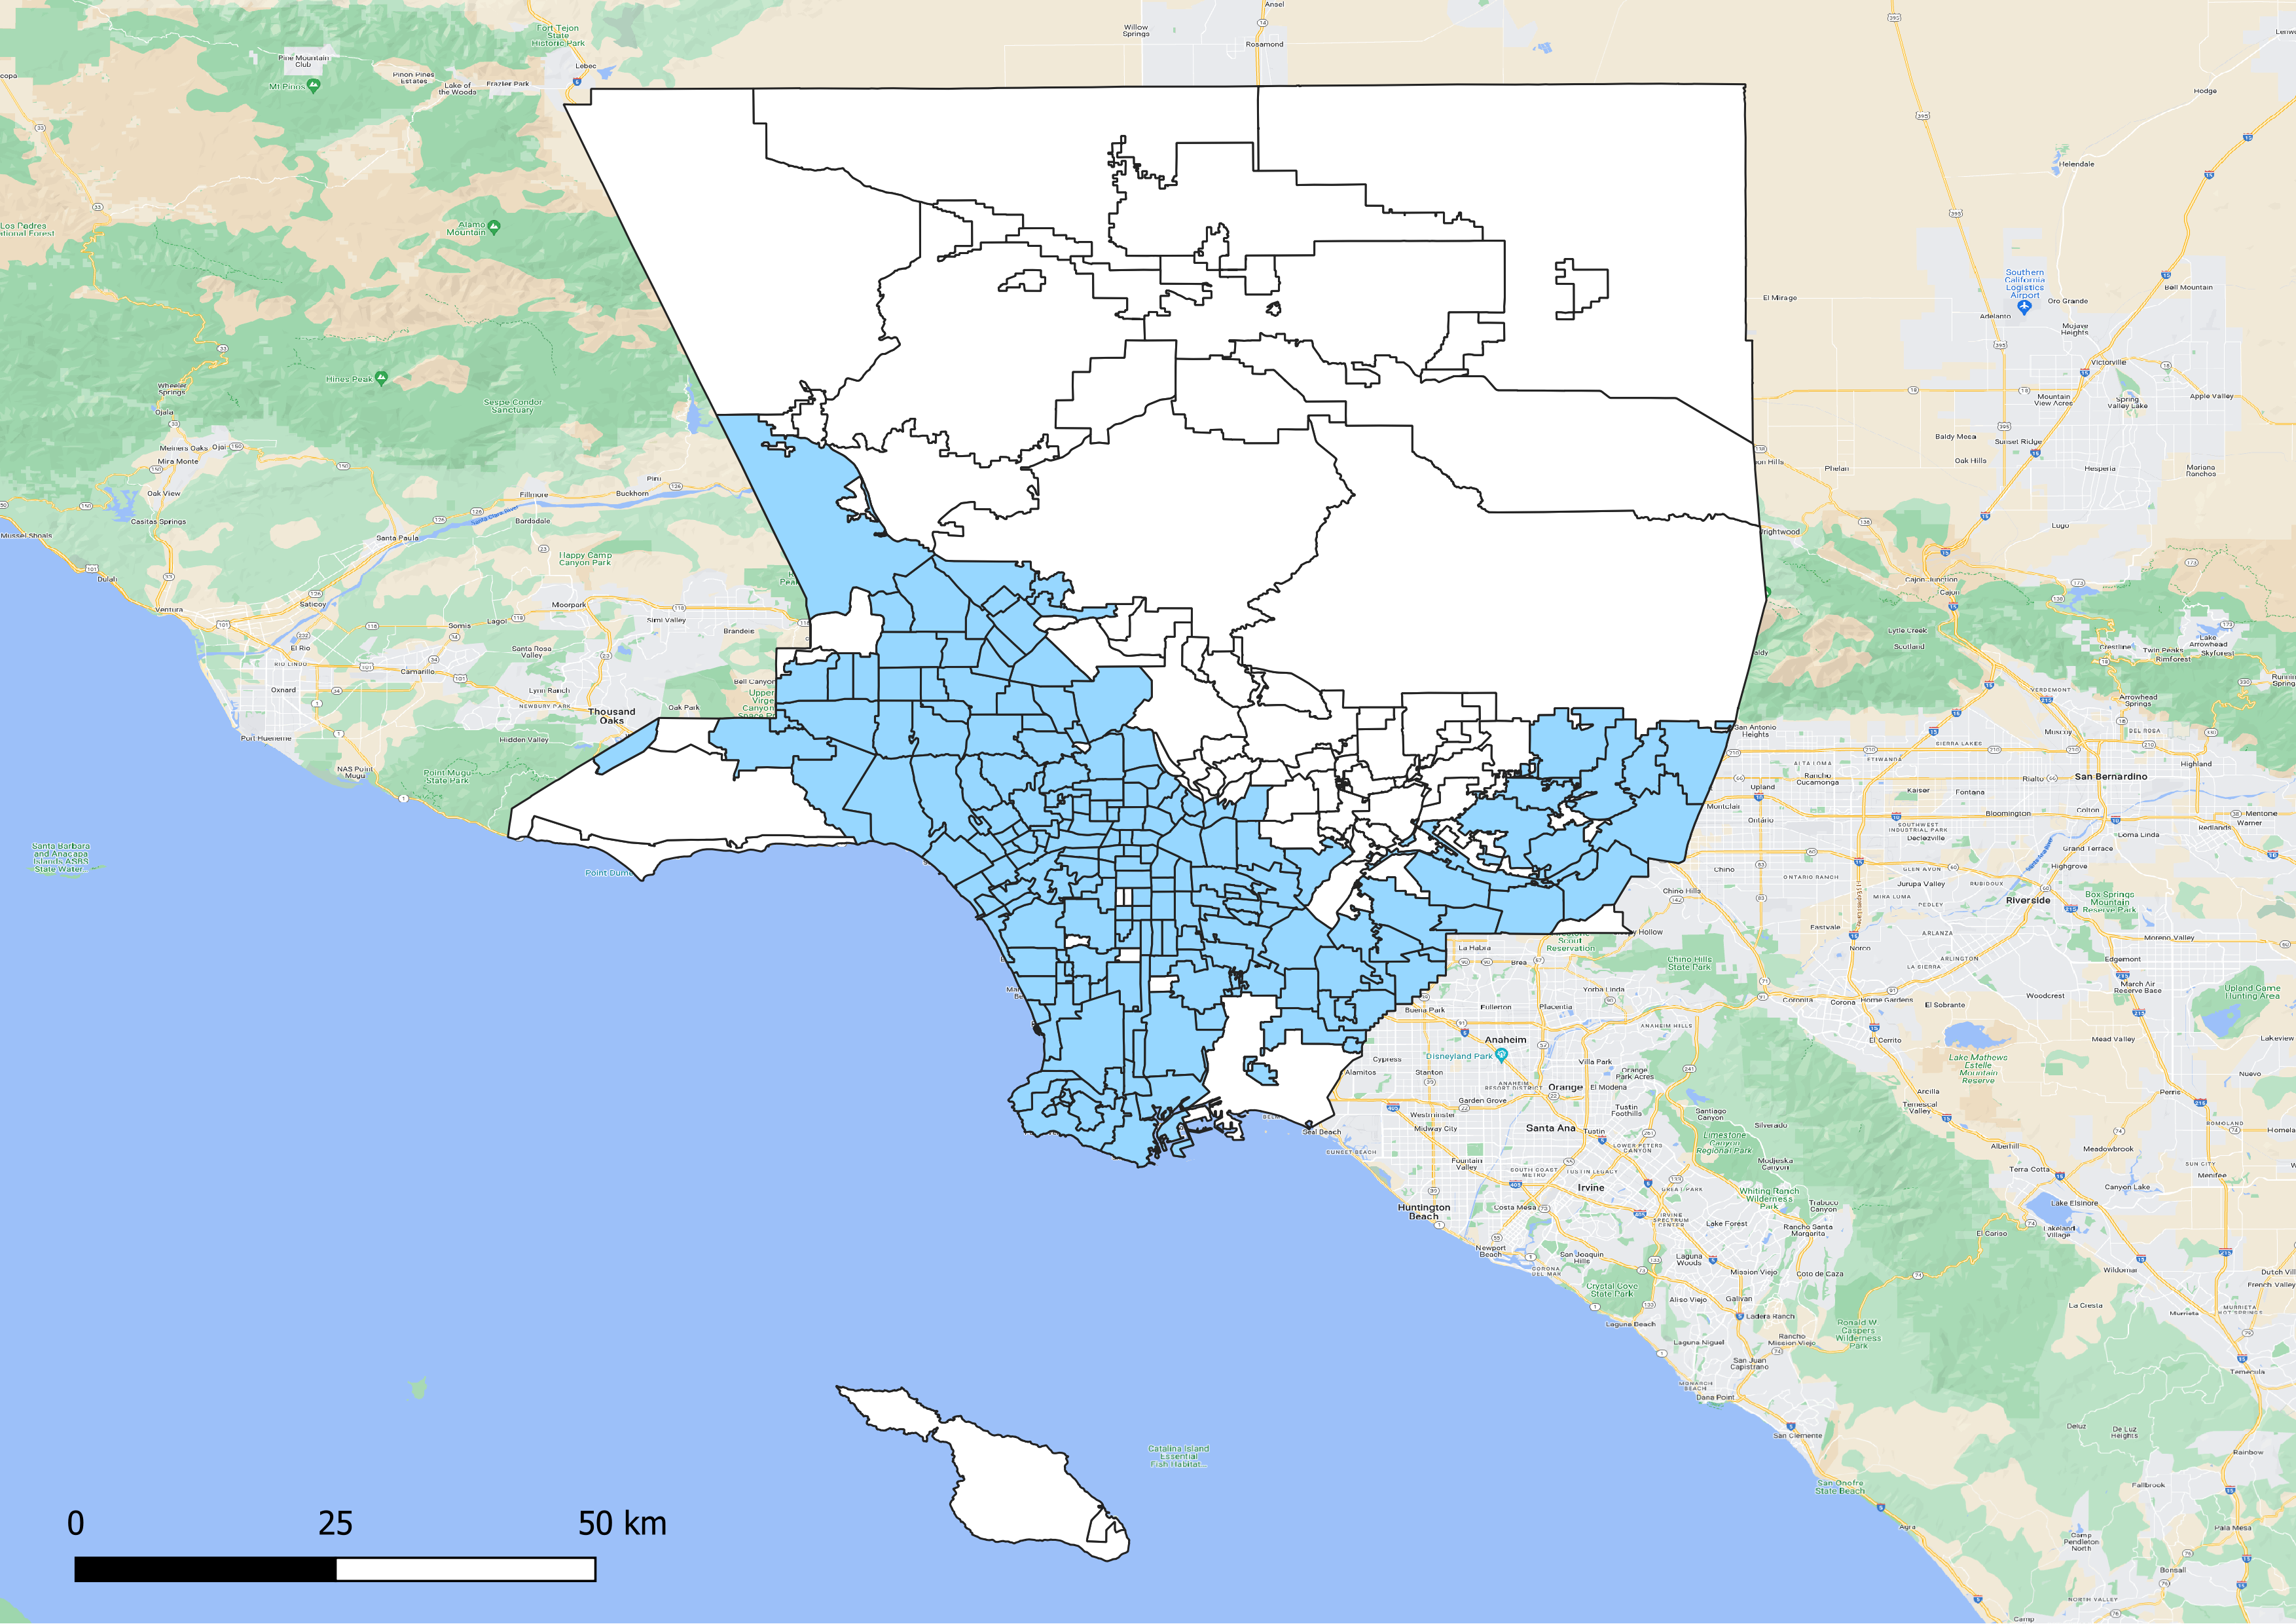
\includegraphics[width=0.8\textwidth]{images/4_materiais/gis/LA_BairrosSelecionados.png}
    \caption*{Fonte: Produzido pelos autores Fernandes \& Alves}
    \label{fig:bairros_LA}
\end{figure}

Vale ressaltar que a peculiaridade de bairros sem operação de entregas resulta do fato de o município de Los Angeles, na região norte, possuir regiões montanhosas e pouco habitadas.
Este fenômeno também está presente no \textit{shapefile} (Figura \ref{fig:GRU_shapefile_QGIS}) da cidade de Guarulhos, sugerindo que, em geral, bairros mais ao centro da cidade geralmente são menores e mais discretizados. 

\subsection{Demais cidades americanas}

Dado que a base de dados operacional da Amazon compõe-se ao longo de cinco grandes regiões metropolitanas nos Estados Unidos: Austin, Boston, Chicago, Los Angeles e Seattle; e, apesar do foco supracitado ao município de Los Angeles, também buscou-se obter dados georreferenciados das outras 4 cidades. 
%
Para tal, repetiu-se o processo citado anteriormente para Los Angeles cidade a cidade, buscando o mapeamento dos bairros das cidades em fontes oficiais, tais como prefeituras, governos estaduais, universidades e institutos. No caso de Austin, Texas, o mapeamento foi obtido através de \citeonline{Austin2022}. Já os bairros de Boston foram obtido em \citeonline{BPDA2020}. No caso de Chicago, a prefeitura disponibilizou os dados em \citeonline{Chicago2022}. E, por fim, os bairros de Seattle foram obtidos em \citeonline{Seattle2021}.
Por fim, obtém-se uma relação de polígonos que descrevem bairro a bairros os municípios das 5 cidades.

%%%%%%%%%%%%%%%%%%%%%%%%%%%%%%%%%%%%%%%%%%%%%%
\section{Geoestatísticas} \label{GeoDa}

Através do \textit{GeoDa}, buscou-se estabelecer procedimentos que permitissem análises geoespaciais de dados, como por exemplo análises referentes à autocorrelação espacial, conforme descritas na seção \ref{sec:autocorrelacaoEsp}.
%
Para que se utilize tal análise, é necessário que os dados estudados sejam organizados numa estrutura de zonas. 
Assim, como supracitado na Seção \ref{sec:dados_de_informacao_geografica}, é possível estruturar a região estudada em bairros.

Em seguida define-se as diferentes variáveis a serem estudadas. 
Como já apresentado no tópico \ref{sec:variaveis_do_problema}, considera-se, ao longo do trabalho, as variáveis Repasse, devolução e NAS, obtendo-se a o valor de cada variável em cada zona e, em sequência, pode-se construir a análise de Moran citada.
%
Tal construção produz um mapa LISA e um gráfico de dispersão para cada variável estudada (percentual de repasses, devoluções e NAS).

Maiores detalhes acerca dos conceitos por trás das ferramentas e teorias utilizadas no GeoDa por ser encontrados na Seção \ref{sec:autocorrelacaoEsp}.

%%%%%%%%%%%%%%%%%%%%%%%%%%%%%%%%%%%%%%%%%%%%%%
\section{Dispersão geográfica das rotas} \label{sec:dispGeoRotas}

Para quantificar a composição geográfica das rotas, optou-se por construir uma nova medida nomeada ``dispersão geográfica da rota''. 
Sua concepção baseia-se na tese de que clientes mais segregados do resto dos clientes de uma mesma rota podem apresentar um comportamento diferente dos demais. 
Tal tese é estruturada na ideia de que a equipe de entregas da rota em questão pode oferecer um tratamento particular a PDEs localizados à parte da maioria dos PDEs de tal rota.

Assim, para cada rota, calcula-se a distância de todos os PDEs que a compõe entre si. 
Em sequência, calcula-se a média das distância para cada PDE, em cada rota.
Desta forma, é possível mensurar o quão longe cada PDE está dos outros PDEs da mesma rota.
Posteriormente, assume-se que há uma distribuição normal de probabilidade dessas distâncias médias em cada rota, para que se possa identificar quais PDEs estão mais à deriva da distribuição espacial e, por consequência, estão localizados na região da ``cauda'' da distribuição normal. 
Para tal, utilizou-se a normalização da variável distância à Distribuição Normal Padronizada (Z). 

Tal divisão pode ser exemplificada nas Figuras \ref{fig:AMBEV_Compac_1}, \ref{fig:AMBEV_Compac_2} e \ref{fig:AMBEV_Compac_3}, advindas do teste da metodologia na base de dados da empresa de bebidas.
Nelas, observa-se a composição de PDEs de duas rotas distintas.
Os PDEs são coloridos de forma a identificar, no corte de 95\% de significância, os que são considerados marginais (vermelho) e os que não são (azul). 

\begin{figure}[H]
    \centering
     \caption{Exemplos de rotas segregadas entre marginais e não-marginais.}
     \begin{subfigure}{.3\textwidth}
         \centering
         \caption{Exemplo 1.}
         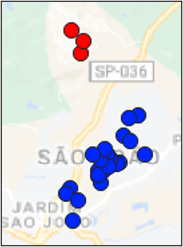
\includegraphics[height=1.2\textwidth]{images/4_materiais/compactacao/CompactacaoExemplo1.png}
         \label{fig:AMBEV_Compac_1}
     \end{subfigure}
     \begin{subfigure}{.3\textwidth}
       \centering
       \caption{Exemplo 2.}
       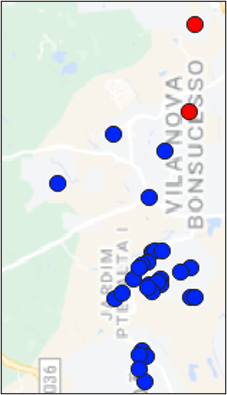
\includegraphics[height=1.2\textwidth]{images/4_materiais/compactacao/CompactacaoExemplo2.png}
       \label{fig:AMBEV_Compac_2}
     \end{subfigure}
     \begin{subfigure}{.3\textwidth}
       \centering
       \caption{Exemplo 3.}
       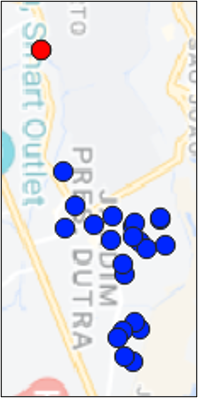
\includegraphics[height=1.2\textwidth]{images/4_materiais/compactacao/CompactacaoExemplo3.png}
       \label{fig:AMBEV_Compac_3}
     \end{subfigure}
     \caption*{\ Fonte: Produzido pelos autores Fernandes \& Alves}
     % \small\textsuperscript{} Observação: As figuras foram rotacionadas para melhor visualização.
 \end{figure}